\documentclass[11pt]{article}

\usepackage[a4paper]{geometry}
\geometry{left=2.0cm,right=2.0cm,top=2.5cm,bottom=2.5cm}

\usepackage{ctex} % 支持中文的LaTeX宏包
\usepackage{amsmath,amsfonts,graphicx,subfigure,amssymb,bm,amsthm,mathrsfs,mathtools,breqn} % 数学公式和符号的宏包集合
\usepackage{algorithm,algorithmicx} % 算法和伪代码的宏包
\usepackage[noend]{algpseudocode} % 算法和伪代码的宏包
\usepackage{fancyhdr} % 自定义页眉页脚的宏包
\usepackage[framemethod=TikZ]{mdframed} % 创建带边框的框架的宏包
\usepackage{fontspec} % 字体设置的宏包
\usepackage{adjustbox} % 调整盒子大小的宏包
\usepackage{fontsize} % 设置字体大小的宏包
\usepackage{tikz,xcolor} % 绘制图形和使用颜色的宏包
\usepackage{multicol} % 多栏排版的宏包
\usepackage{multirow} % 表格中合并单元格的宏包
\usepackage{pdfpages} % 插入PDF文件的宏包
\RequirePackage{listings} % 在文档中插入源代码的宏包
\RequirePackage{xcolor} % 定义和使用颜色的宏包
\usepackage{wrapfig} % 文字绕排图片的宏包
\usepackage{bigstrut,multirow,rotating} % 支持在表格中使用特殊命令的宏包
\usepackage{booktabs} % 创建美观的表格的宏包
\usepackage{circuitikz} % 绘制电路图的宏包
\usepackage{tabularx}
\usepackage{titlesec}

% 设置代码块样式
\definecolor{dkgreen}{rgb}{0,0.6,0}
\definecolor{gray}{rgb}{0.5,0.5,0.5}
\definecolor{mauve}{rgb}{0.58,0,0.82}
\lstset{
  frame=tb,
  aboveskip=3mm,
  belowskip=3mm,
  showstringspaces=false,
  columns=flexible,
  framerule=1pt,
  rulecolor=\color{gray!35},
  backgroundcolor=\color{gray!5},
  basicstyle={\small\ttfamily},
  numbers=none,
  numberstyle=\tiny\color{gray},
  keywordstyle=\color{blue},
  commentstyle=\color{dkgreen},
  stringstyle=\color{mauve},
  breaklines=true,
  breakatwhitespace=true,
  tabsize=3,
}

% 轻松引用, 可以用\cref{}指令直接引用, 自动加前缀. 
% 例: 图片label为fig:1
% \cref{fig:1} => Figure.1
% \ref{fig:1}  => 1
\usepackage[capitalize]{cleveref}
% \crefname{section}{Sec.}{Secs.}
\Crefname{section}{Section}{Sections}
\Crefname{table}{Table}{Tables}
\crefname{table}{Table.}{Tabs.}

% 设置标题格式
\titleformat{\section}
  {\bf\large}{\thesection}{1em}{}
\titleformat{\subsection}
  {\normalfont}{\thesubsection}{1em}{}


\renewcommand{\emph}[1]{\begin{kaishu}#1\end{kaishu}}

%改这里可以修改实验报告表头的信息
\newcommand{\name}{李华}
\newcommand{\studentNum}{0000000}
\newcommand{\major}{物理学}
\newcommand{\group}{A组}
\newcommand{\dateYear}{20xx}
\newcommand{\dateMonth}{xx}
\newcommand{\dateDay}{xx}

\newcommand{\experiName}{将大象装进冰箱}


\begin{document}
% 设置行距
\baselineskip=18pt
%页眉
\pagestyle{fancy}
\lhead{基础物理实验报告}
\chead{}
\rhead{\experiName}

\begin{center}
    \huge \heiti 《基础物理实验II》课程实验报告
\end{center}

\begin{flushleft}
    \noindent 姓名:{\makebox[6em][c]{\name}} 学号:{\makebox[6em][c]{\studentNum}}  专业:{\makebox[18em][c]{\major}}\\
    组别:{\makebox[6em][c]{\group}}实验时间:周四上午\enspace{\makebox[3em][c]{\dateYear}}年
    {\makebox[2em][c]{\dateMonth}}月
    {\makebox[2em][c]{\dateDay}}日\\
    实验名称:{\makebox[15em][c]{\experiName}}
    {\noindent}\\
    \rule[4pt]{17cm}{0.1em}
\end{flushleft}
\begin{center}
    \LARGE \bf \experiName
\end{center}

\section{目的要求}

\begin{enumerate}
    \item 掌握冰箱的使用
    \item 掌握大象的搬运
\end{enumerate}

\section{仪器用具}
\section{实验原理}
带编号的公式
\begin{equation}
        u_{C}=\frac{Q}{C}=\frac{1}{C}\int{i_{2}\mathrm{d}t}=\frac{1}{CR_{2}}\int{u_{R_{2}}\mathrm{d}t}\approx \frac{1}{CR_{2}}\int{u_{2}\mathrm{d}t}
    \end{equation}
\section{实验步骤}
    \subsection{掌握冰箱的使用}
        \begin{enumerate}
          \item[1)] 掌握冰箱的使用\\
          
        \end{enumerate}
\section{数据处理}

\subsection{原始数据}

    \begin{table}[h]
  \centering
  \begin{tabular}{lccc} % 第一列左对齐，后三列居中
    \toprule
    组别 & 测量1  & 测量2  & 测量3  \\
    \midrule
    aaa & 95.2 & 94.8 & 95.0 \\
    bbb & 93.5 & 92.1 & 92.8 \\
    ccc & 96.1 & 95.5 & 95.8 \\
    \bottomrule
  \end{tabular}
  \caption{原始数据表格(cm)}
\end{table}

\subsection{直接测量数据处理}
算数平均值 $\bar{x} = 19.982 \enspace\text{cm}$

样本标准偏差 $\sigma_{\bar{x}} = \sqrt{\dfrac{\sum_{i=1}^{n}(x_i - \bar{x})^2}{n-1}} =0.092 \enspace\text{cm}$

算术平均值的标准偏差 $\bar{\sigma}_x = \dfrac{\sigma_x}{\sqrt{n}} = 0.038 \enspace\text{cm}$

A类标准不确定度 $u_a = t_{(0.683,5)} \cdot \sigma_{\bar{x}} = 0.042 \enspace\text{cm}$

B类标准不确定度 $u_b = \dfrac{\varepsilon_x}{\sqrt{3}} = 0.058 \enspace\text{cm}$

合成不确定度 $u_L = \sqrt{u_a^2+u_b^2} \approx 0.07 \enspace\text{cm}$\\

最终结果：$L=(19.98\pm 0.07) \enspace\text{cm}$

同理可得……

\subsection{间接测量数据处理}

   例一：推导不确定度合成公式
   $$ u_V = \sqrt{\sum_i \left( \frac{\partial f}{\partial x_i} u_{x_i} \right)^2 } =\dots=0.080 \enspace\text{cm}^3$$
   
   例二：取对数 $\ln g=\ln(4\pi^2)+\ln l-2\ln T$，则相对不确定度
    $$ u_g=g\cdot\sqrt{\sum_{i}(\frac{\partial\ln g}{\partial x_i}u_{x_i})^2}=\dots=\dots\enspace\text{m/s}^2$$


\subsection{拟合/分析数据图表插入}
\begin{figure}[H]
    \centering
    \subfigure[并排图片示例1]{
        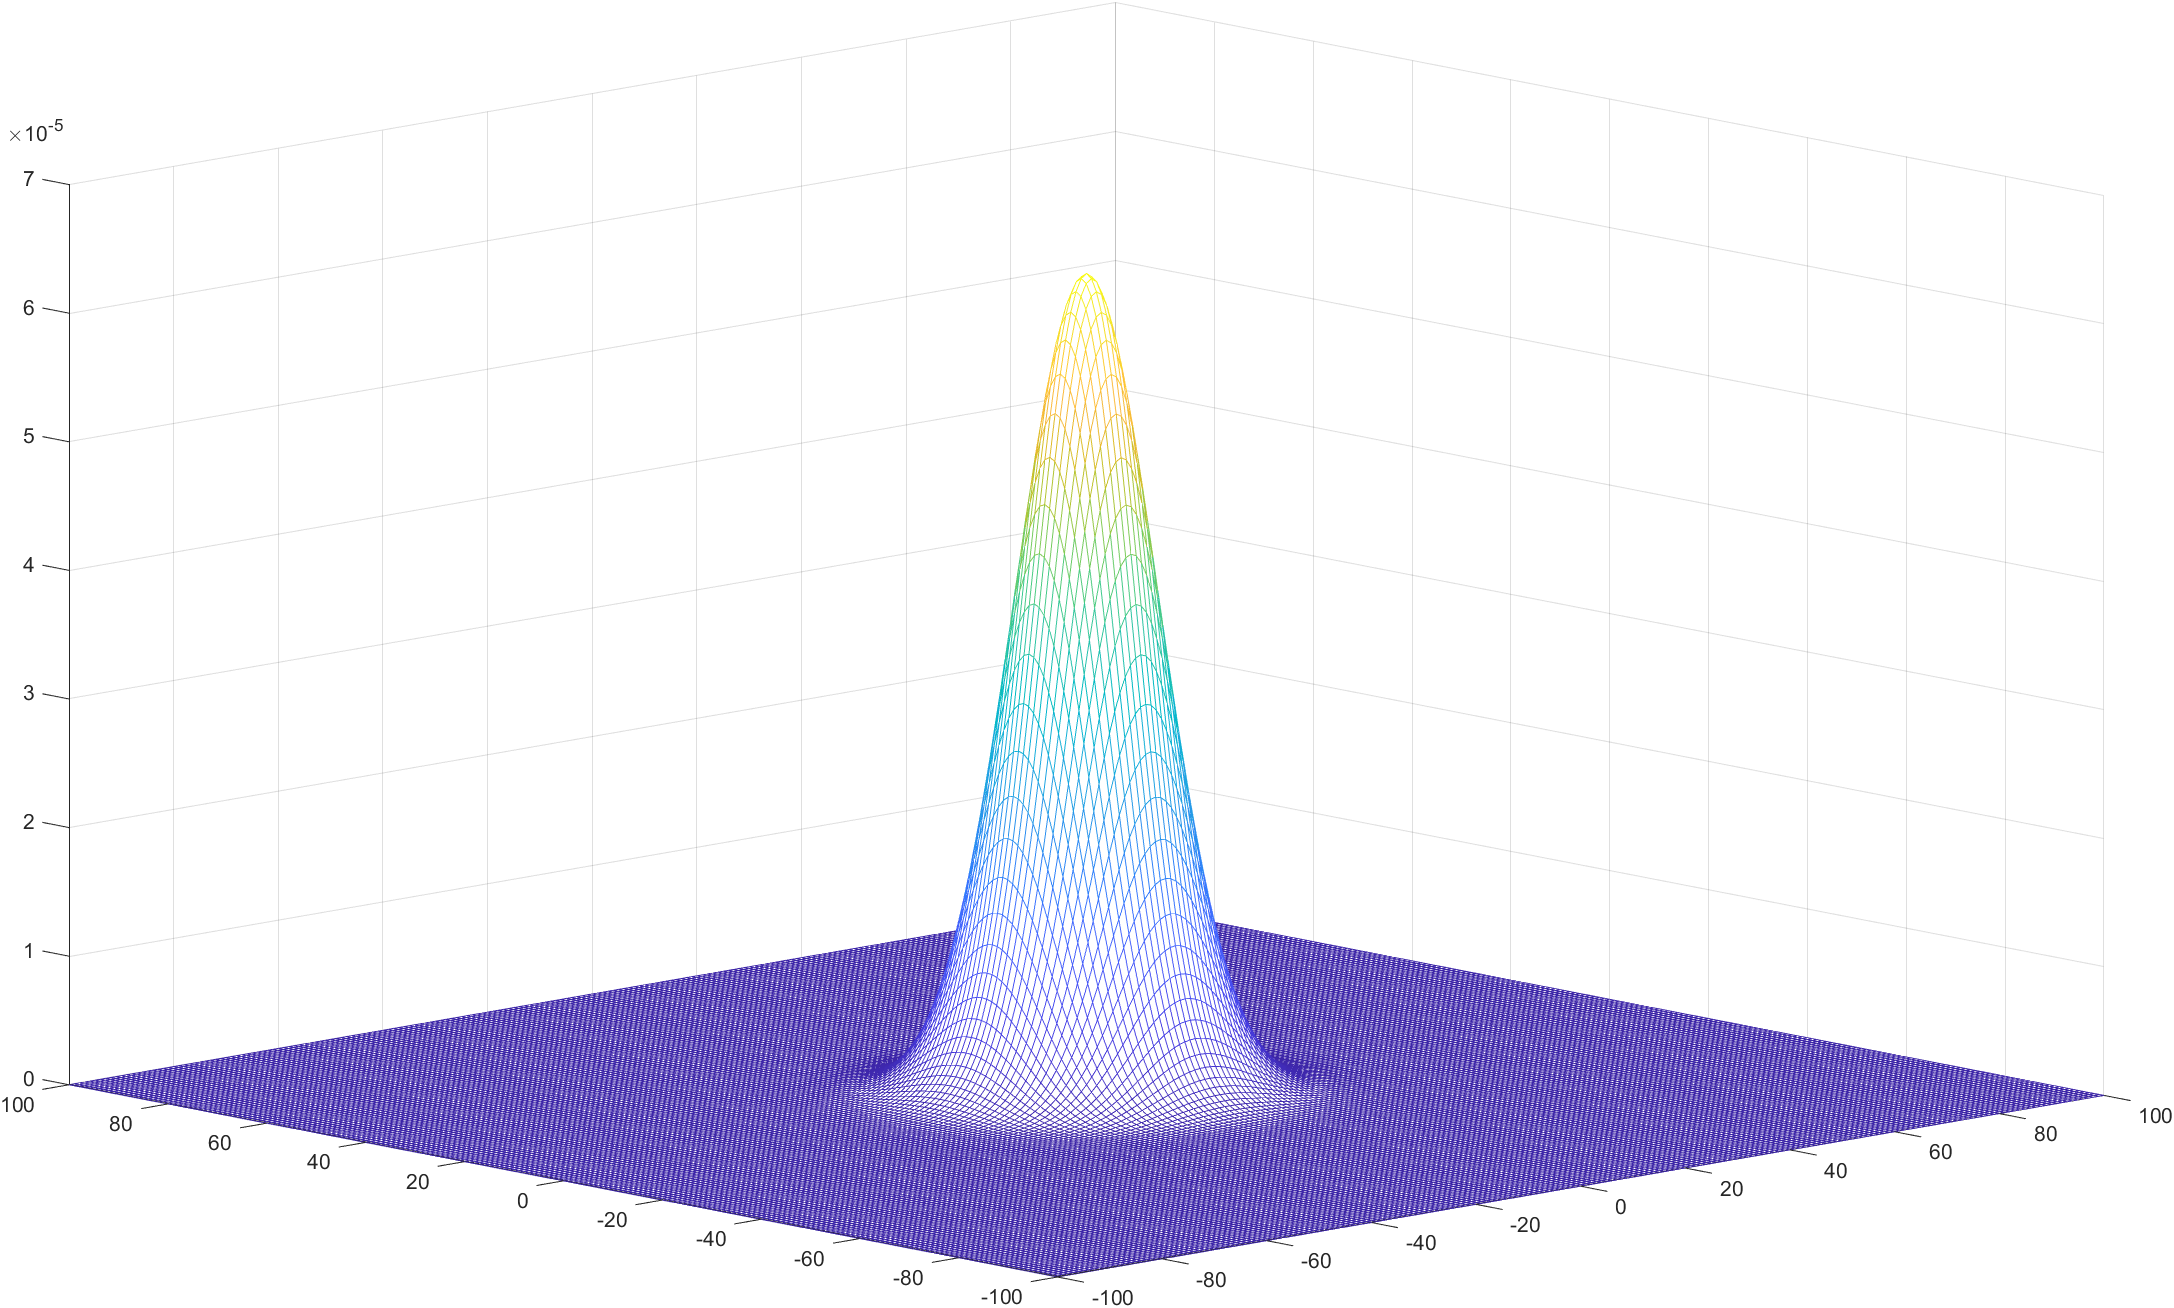
\includegraphics[width=7.5cm]{Fig/Gaussian.png}}
    \hspace{0.5in}
    \subfigure[并排图片示例2]{
        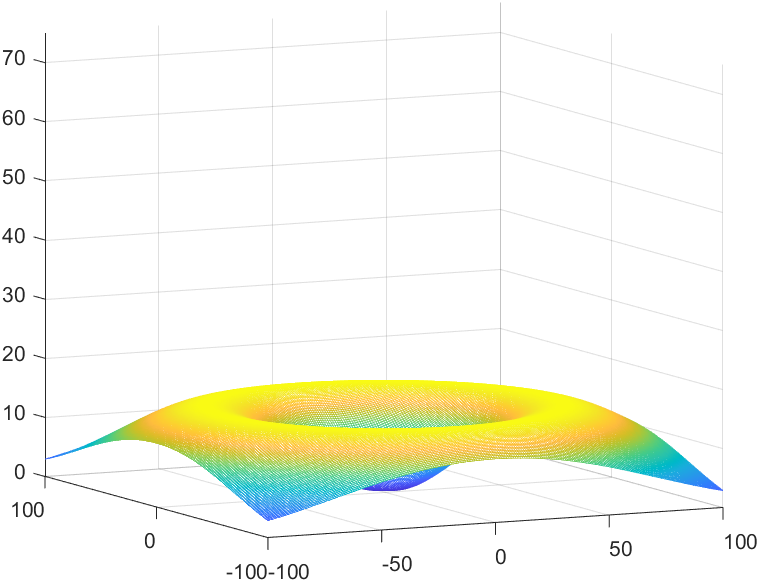
\includegraphics[width=7.5cm]{Fig/Maxwell.png}}
    \hspace{0.5in}
    \caption{并排图片}
\end{figure}

\section{问题讨论与思考题}

\section{总结}

\end{document}